% ----- INPUT
\newcommand{\rsimagew}{0.95\textwidth}
\newcommand{\rsimageh}{0.62875 * \textwidth}

\newcommand{\rsshift}{-0.4}


\begin{tikzpicture}[
        arr/.style = { -{Stealth[ ]} },
        bluearrow/.style = {arr, draw=third-color, fill=third-color, thick},
        blackarrow/.style = {arr, ultra thick},
    ]
    
    
    \begin{scope}
        \node[anchor=south west,inner sep=0] at (0,0) {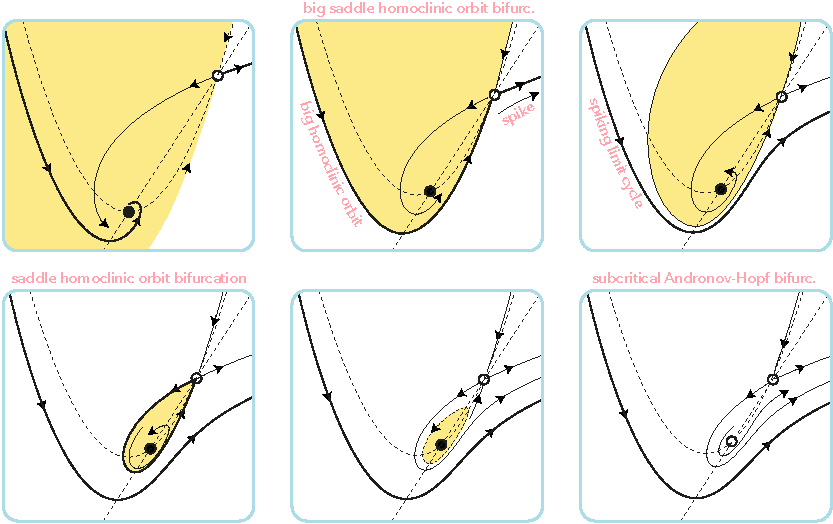
\includegraphics[width=\rsimagew]{src/assets/images/rs-bifurcations.pdf}};
    \end{scope}
    
    \begin{scope}
        
        \node[shift={(\rsshift, 0)}, rotate=90] at (0, 0.5 * \rsimageh) {Recovery variable $r$};
        
        \node[shift={(0, \rsshift)}] at (0.5 * \rsimagew, 0) {Membrane potential $p$};
        
    \end{scope}
        
\end{tikzpicture}